\section{Model}

%Each interaction then has a set of periods $d \in D_{ij}$ each with a start time $a_d$, an end time $b_d$, and a rate $\lambda_d$.
%Consider a nonhomogeneous Poisson process with  intensity $\lambda(t)$ that is piecewise constant with respect to a set of knots $\tau$.  We can then write the likelihood of $M$ events $\mathcal{A} = (t_1, \ldots, t_M)$ with $t_m > 0$ as
Consider a sequence of events $\mathcal{A} = (0,t_1, \ldots, t_M)$ arising from a nonhomogeneous Poisson process with  intensity $\lambda(t)$.
If the intensity is left continuous and piecewise constant with respect to a set of knots $\tau$ then the likelihood can be written
\begin{align}
\mathcal{L}(\mathcal{A}|\theta) &= \prod_{m=1}^M \lambda(t_m) \exp\left\{ - \int_{0}^{t_M} \lambda(s)ds \right\} \notag  \\
&= \prod_{m=1}^M \lambda(t_m) \prod_{k=1}^{|\tau|} \exp\left\{ - (\tau_{k} - \tau_{k-1}) \lambda(\tau_k) \right\}%  \exp\left\{ - (t - \tau_{M}) \lambda(t) \right\}
\end{align}
%\noindent where the $m$th event occurs at time $t_m$, the intensity function $\lambda(t)$ is left continuous, and each $\tau_k \in [0,t_M]$.

% \begin{align}
% \mathcal{L}(A|\theta) &= \prod_{m=1}^M \lambda_{i_m}(t_m|\cdot) \prod_{i \in \mathcal{R}}  \exp\left\{ - \int_{0}^{t_M} \lambda_{i}(\tau | \cdot)d\tau \right\} \\
% &= \prod_{m=1}^M \lambda_{i_m}(t_m|\cdot) \prod_{i \in \mathcal{R}} \prod_{v \in D_{i}} \exp\left\{ - (b_v - a_v) \lambda_{i}(b_v | \cdot ) \right\}
% \end{align}

One can extend the above to marked point processes where each event contains additional information.
In the context of relational events occurring among $N$ nodes, each event in the process contains both a sender $i$ and a recipient $j$ such that  $(i,j) \in \mathcal{R}$, where $\mathcal{R}$ is the \emph{risk set} comprised of all allowed dyads.
We assume each dyad $(i,j) \in \mathcal{R}$ occurs as a Poisson process with intensity $\lambda_{ij}(t|\cdot)$ that is piecewise constant and depends on the previous history of events  $\mathcal{A}_t = \{(t_m,i_m,j_m): t_m \in [0,t) \}$.
The likelihood of an observed event history $\mathcal{A}_{t_M}$ (also denoted $\mathcal{A}$ for convenience) is
\begin{align}
\mathcal{L}(\mathcal{A}|\theta) &= \prod_{m=1}^M \lambda_{i_m,j_m}(t_m|\cdot) \prod_{(i,j) \in \mathcal{R}}\exp\{ - (t_m - t_{m-1}) \lambda_{ij}(t_m | \cdot) \}
\label{eqn:llk}
\end{align}
%\prod_{(i,j) \in \mathcal{R}}\exp\{ - (t - t_{M}) \lambda_{ij}(t | \cdot) \}.

\begin{figure}
\centering
\begin{minipage}[b]{0.45\linewidth}
  \begin{tikzpicture}[scale=.8,transform shape,thick]
    \node[vertex] (n1) at (0,0)  {1};
    \node[vertex] (n2) at (2,2)  {2};
    \node[vertex] (n3) at (4,0) {3};
    \node[vertex] (n4) at (2,-2) {4};
    \draw[-stealth] (.4,.4) -- (1.6,1.6);
    \draw[-stealth] (2.4,1.6) -- (3.6,.4);
    \node at (.7,1.1) {$t_1$};
    \node at (3.3,1.1) {$t_2$};
  \end{tikzpicture}
  \caption{Dynamic network data}
\end{minipage}
\begin{minipage}[b]{0.45\linewidth}
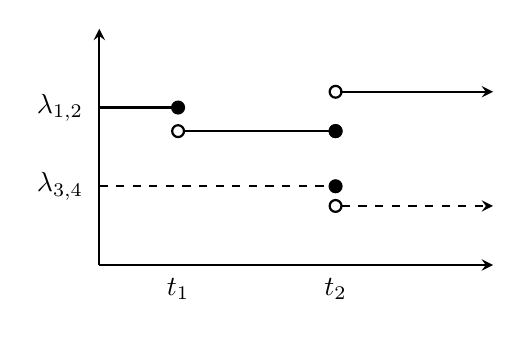
\begin{tikzpicture}[scale=1,transform shape,thick]
\draw[-stealth] (0,0) -- (0,3);
\draw[-stealth] (0,0) -- (5,0);

% First timeline
\draw (0,2) -- (1,2);
\draw[fill=black] (1,2) circle (0.75mm);
\draw (1,1.7) circle (0.75mm);
\draw (1.08,1.7) -- (3,1.7);
\draw[fill=black] (3,1.7) circle (0.75mm);
\draw (3,1.7) circle (0.75mm);
\draw (3,2.2) circle (0.75mm);
\draw[-stealth] (3.05,2.2) -- (5,2.2);

% second timeline
\draw[dashed] (0,1) -- (3,1);
\draw[fill=black] (3,1) circle (0.75mm);
\draw (3,.75) circle (0.75mm);
\draw[dashed, -stealth] (3.08,.75) -- (5,.75);

% labels
\node at (-.5,2) {$\lambda_{1,2}$};
\node at (-.5,1) {$\lambda_{3,4}$};
\node at (1,-.3) {$t_1$};
\node at (3,-.3) {$t_2$};
\end{tikzpicture}
\caption{Intensities for two dyads}
\end{minipage}
\caption[]{Illustration of event data and the assumptions of the model.  Left: An sequence of two events among four nodes: (1,2) occurs at time $t_1$ and (2,3) occurs at time $t_2$.  Right: The intensity functions $\lambda_{1,2}(t)$ (solid) and $\lambda_{34}(t)$ (dotted).  We assume $\lambda_{34}$ can only change after events sent or received by node 3.\footnotemark }
\label{fig:example}
\end{figure}

\footnotetext{TODO? Illustration of the block model, where events in cluster 1 (circles) are governed by the vector $\beta_{1,1}$, events in cluster 2 (squares) are governed by $\beta_{2,2}$, and an circle-to-square event governed by $\beta_{1,2}$.}


% \begin{figure}
%  \def\svgwidth{6in}
%   \input{example1.pdf_tex}
% \caption{Illustration of event data and the assumptions of the model.  Left: An sequence of two events among four nodes: (1,2) occurs at time $t_1$ and (2,3) occurs at time $t_2$.  Center: The intensity functions $\lambda_{1,2}(t)$ (solid) and $\lambda_{34}(t)$ (dotted).  Note $\lambda_{34}$ can only change when events occur involving either node 3 or node 4.  Right: Illustration of the block model, where events in cluster 1 (circles) are governed by the vector $\beta_{1,1}$, events in cluster 2 (squares) are governed by $\beta_{2,2}$, and an circle-to-square event governed by $\beta_{1,2}$.}
% \label{fig:example}
% %\includegraphics[width=6in]{example}
% \end{figure}

%This implies that  $\mathcal{R}_{i,j}$ is the set of dyads involving either $i$ or $j$ and that we will only use  statistics $\mathbf{s}(t,i,j)$ that do not change until an event involving either $i$ or $j$ occurs.

We aim to learn about the dynamics between subsets of nodes.   To facilitate this, we assume each node $i$ is assigned a latent cluster $z_i$ and use a log linear model for the intensity functions
\begin{align*}
\log \lambda_{ij}(t | \mathcal{A}_t,\mathbf{\beta},\mathbf{z}) &= \boldsymbol{\beta}'_{z_i,z_j} \mathbf{s}(t,i,j,\mathcal{A}_t)
%z_i &\sim \mbox{CRP}(\alpha) &
%\boldsymbol{\beta}_{k,l} &\sim %\mbox{N}_p(\boldsymbol{\mu},\boldsymbol{\sigma}^2I)
\end{align*}
where for each pair of clusters $(k,l)$ we have a vector of parameters $\boldsymbol{\beta}_{k,l} \sim \mbox{N}_P(\boldsymbol{\mu},\boldsymbol{\sigma}^2I)$ that corresponds to the vector of $P$ statistics $\mathbf{s}(t,i,j,\mathcal{A}_t)$ computed from the previous history $\mathcal{A}_t$.
Thus, our model for the rate of $(i,j)$ events has the same parameters as for other dyads occurring between group $z_i$ and $z_j$.

 In practice we may believe an interaction between one dyad should not affect the rate of an entirely separate dyad.
As shown in Figure \ref{fig:example}, we allow each intensity function $\lambda_{ij}(t)$ to only change following an event where $i$ was the sender or the recipient.
This is sensible in distributed settings where $i$ has limited knowledge about interactions among other actors.
In the Appendix we show how this assumption also reduces the computational complexity of computing the above likelihood.\footnote{This is analogous to a Markov condition for this class of models.}

We allow the blocks to share information by placing a hierarchical prior on the collection of $\boldsymbol{\beta}_{k.l}$ where $\mu_p \sim N(0,1)$ and $\sigma_p^2 \sim \mbox{Inv-Gamma}(3,1)$.
The cluster assignments are given a non-parameteric priors $z_i \sim \mbox{CRP}(\alpha)$.

\subsection{Model specification}

\begin{table}[t]
\footnotesize
\center
\begin{tabular}{|l|l|}
\hline
Statistic & Formula \\
\hline
\hline
Intercept& $s_{0}(t,i,j) = 1$\\
Reciprocity (AB-BA)& $s_{1}(t,i,j) = I(i_m=i,j_m=j,i_{v_{mij}}=j,j_{v_{mij}}=i)$\\
Turn-continuing (AB-AY)& $s_{2}(t,i,j) =  I(i_m=i,j_m=j,i_{v_{mij}}=i,j_{v_{mij}}\ne j)$\\
Turn-taking (AB-BY)&$s_{3}(t,i,j) = I(i_m=i,j_m=j,i_{v_{mij}}=j,j_{v_{mij}}\ne i)$\\
%Turn-usurping (AB-XA)& $s_{7}(t,i,j) = I(i_m=i,j_m=j,i_{v_{mij}} \ne j,j_{v_{mij}}=i)$\\
%Turn-usurping (AB-XB)&$s_{8}(t,i,j) = I(i_m=i,j_m=j,i_{v_{mij}} \ne i,j_{v_{mij}}=j)$\\
Sender out-degree& $s_{4}(t,i,j) = f(\sum_{m:t_m<t} I(i_m=i) )$\\
Sender in-degree& $s_{5}(t,i,j) = f(\sum_{m:t_m<t} I(j_m=i) )$\\
Dyad count& $s_{6}(t,i,j) = f(\sum_{m:t_m<t} I(i_m=i,j_m=j) )$\\
%Receiver out-degree& $s_{3}(t,i,j) = f(\sum_{m:t_m<t} I(i_m=j))$\\
%Receiver in-degree& $s_{4}(t,i,j) = f(\sum_{m:t_m<t} I(j_m=j))$\\
\hline
\end{tabular}
\label{tab:stats}
\caption{Statistics used to specify intensity functions using the previous history $\mathcal{A}_t$.}
\end{table}



In Table \ref{tab:stats} we list the statistics we use in our experiments for  $\mathbf{s}(t,i,j)$.
Several statistics use $v_{mij} \in [0,M]$, the index of the last event where $(i,j)$ occurred.  % (n.b. $t_{v_{mij}} = \tau_{mij}$).
If $(i,j)$ has never occurred, we set $v_{mij}=0$.  We include degree effects to model possible rich-get-richer phenomenon.
For example, a particular node sending often may indicate they will continue to be a sender in the future.
We normalize these counts by the number of events up until a dyad's prior changepoint.\footnote{This seems to avoid ``explosion'' when simulating from the model.  TODO: Explore the theory about these sorts of statistics.  Aalen has a few suggestions.}
Other statistics could be of interest for particular substantive questions \cite{Butts2008,Vu2011}.  \footnote{Describe the form of $f()$.  Right now it is $f(x) = \log \frac{x+1}{m + N(N-1)}$.}

The next set of statistics are \emph{participation shift} effects inspired by research in conversational norms \cite{Gibson2003}.
For example, an AB-BA effect indicates an increased propensity for reciprocity.
The final set of effects allow one to model phenomenon such as triadic closure.
Though we use only the above statistics in our experiments, one may use any quantity or set of covariates about a given dyad that is computed using the previous history of events.
The only restriction is that the statistic may not change in value between each observed event.\footnote{This prevents one from using the number of events occurring in some previous time window, as in \cite{Gunawardana2011}.}

\subsection{Relation to other models}

Our formulation is reminiscent of the stochastic blockmodel \cite{Nowicki2001,Kemp} which models the probability of a dyad as $p(y_{ij}) =\mbox{logit}^{-1}( \eta_{z_i,z_j})$ where $\eta_{z_i,z_j}$ is interpreted as a mixing rate between group $z_i$ and group $z_j$.
In the proposed method, however, the blockmodel structure facilitates the study of intra-group and inter-group dynamics via a continuous-time network model.

The above framework generalizes several important special cases.
For example,  using only the intercept statistic $s_0(t,i,j) = 1$ is analogous to the stochastic block model for static networks.
Under this model each dyad is a homogeneous Poisson process and all dyad intensities $\lambda_{i,j}$ within block $(z_i,z_j)$ have the same intensity, $\exp\{\boldsymbol{\beta}_{z_i,z_j}\}$.
As these intensities do not change under this specification, the likelihood simplifies to
$$\mathcal{L}(\mathcal{A}|\beta) = \prod_{m=1}^M \lambda_{i_m,j_m} \prod_{(i,j) \in \mathcal{R}} \exp\{-t_M \lambda_{i,j}\}$$

Alternatively, if one models only the order of the events (ignoring the times at which they occur), the likelihood can be written as
\begin{align}
\mathcal{L}_{\mbox{mult}}(\mathcal{A}|\beta) = \prod_{m=1}^M \frac{\lambda_{i_m,j_m}(t_m | \cdot)}{\sum_{(i,j) \in \mathcal{R}} \lambda_{i,j}(t_m | \cdot)}.
\label{eqn:multllk}
\end{align}
The functional form is similar to conditional logit models used for discrete choice data \cite{McFadden1984}, though here the possible choices are all the dyads in $\mathcal{R}$.

